\begin{exercise}
      {ID-b59dad45f332abd522fdd6e2a0586aad0f293bb0}
      {Quadrat}
  \ifproblem\problem
    \begin{minipage}[c]{0.24\linewidth}
      \centering
      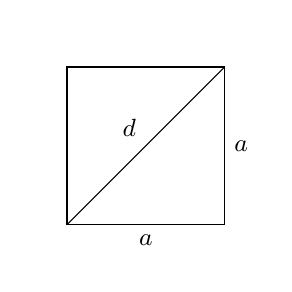
\begin{tikzpicture}
        \clip (-0.5, -0.5) rectangle (2.5, 2.5);
        \draw (0, 0) rectangle (2, 2);
        \draw (0, 0) -- (2, 2);
        \node[below] at (1, 0) {\small$a$};
        \node[right] at (2, 1) {\small$a$};
        \node[above left] at (1, 1) {\small$d$};
      \end{tikzpicture}
    \end{minipage}\hfill
    \begin{minipage}[c]{0.75\linewidth}
      Gib die Seitenlänge $a$ eines Quadrates an, so dass $d$ eine
      natürliche Zahl ist. Begründe, warum kein Quadrat mit natürlicher
      Seitenlänge $a$ eine Diagonale mit rationaler Länge haben kann.
    \end{minipage}
  \fi
  %\ifoutline\outline
  %\fi
  %\ifoutcome\outcome
  %\fi
\end{exercise}
